\section{Systembeschreibung im Zustandsraum}

\subsection{Allgemeine MIMO-Zustandsdarstellung}
\begin{tcolorbox}
\boxtitle{Zustandsdifferentialgleichung und Ausgangsgleichung}
Kontinuierliches Mehrgrößensystem (MIMO) mit Zustandsvektor $\vec{x}(t) \in \mathbb{R}^n$, Eingangsvektor $\vec{u}(t) \in \mathbb{R}^p$ und Ausgangsvektor $\vec{y}(t) \in \mathbb{R}^q$:
\begin{align*}
\dot{\vec{x}}(t) &= A \vec{x}(t) + B \vec{u}(t), \quad \vec{x}(0) = \vec{x}_0 \\
\vec{y}(t) &= C \vec{x}(t) + D \vec{u}(t)
\end{align*}
\begin{itemize}
  \item $A \in \mathbb{R}^{n \times n}$: Systemmatrix (beschreibt innere Dynamik)
  \item $B \in \mathbb{R}^{n \times p}$: Eingangsmatrix (Steuermatrix)
  \item $C \in \mathbb{R}^{q \times n}$: Ausgangsmatrix (Beobachtungsmatrix)
  \item $D \in \mathbb{R}^{q \times p}$: Durchgangsmatrix (direkter Durchgriff)
\end{itemize}
\end{tcolorbox}

\begin{center}
  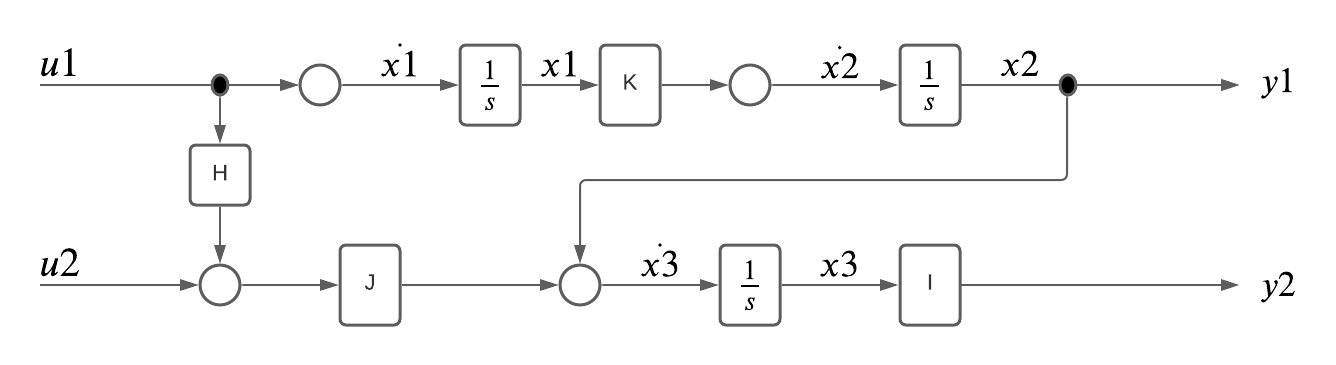
\includegraphics[width=\columnwidth]{images/zustandsraum_bsb.png}
\end{center}

\begin{tcolorbox}
\boxtitle{Pole des Systems / Eigenwerte von $A$}
Die Eigenwerte der Systemmatrix $A$ sind identisch mit den Polen des Systems:
\[
\det(A - sI) \stackrel{!}{=} 0 \implies \text{charakteristisches Polynom}
\]
Das System ist asymptotisch stabil, wenn alle Eigenwerte $\lambda_i$ von $A$ einen echt negativen Realteil besitzen ($\text{Re}\{\lambda_i\} < 0$).
\end{tcolorbox}

\subsection{Polfestlegung durch Zustandsrückführung}
\begin{tcolorbox}
\boxtitle{Vollständige Zustandsrückführung}
\begin{center}
  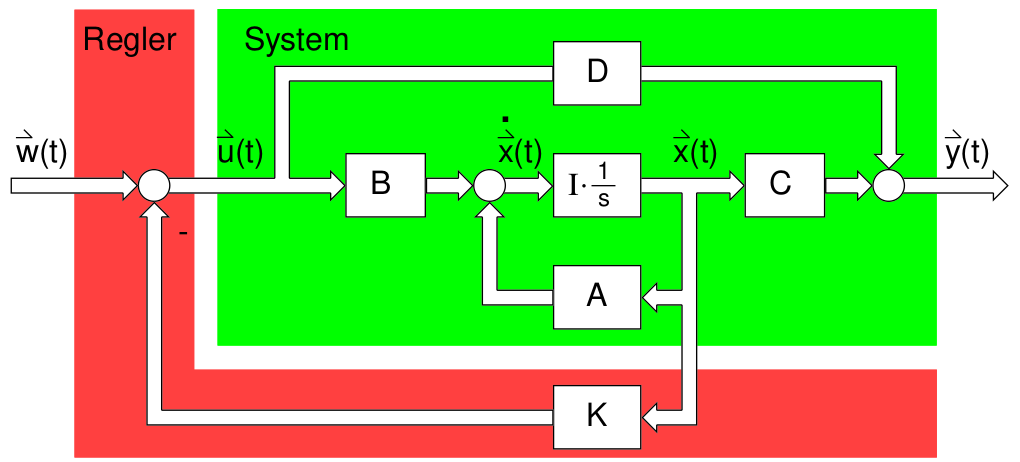
\includegraphics[width=\columnwidth]{images/zustandsrueckfuehrung.png}
\end{center}
Rückführung aller Zustandsgrößen über die Rückführmatrix $K \in \mathbb{R}^{p \times n}$:
\[
\vec{u}(t) = \vec{w}(t) - K \cdot \vec{x}(t)
\]
Einsetzen in die Zustandsdifferentialgleichung:
\[
\dot{\vec{x}}(t) = (A - B K) \vec{x}(t) + B \vec{w}(t)
\]
\textbf{Neue geschlossene Systemmatrix:}
\[
A_{\text{RK}} = A - B K
\]
\end{tcolorbox}

\begin{tcolorbox}
\boxtitle{Polplatzierung durch Koeffizientenvergleich}
Ist das System vollständig steuerbar ($\text{Rang}[B, AB, \dots, A^{n-1}B] = n$), so können durch freie Wahl der Koeffizienten von $K$ alle $n$ Pole des geschlossenen Systems \textbf{vollkommen frei} platziert werden:
\[
\det(A_{\text{RK}} - sI) = \det(A - BK - sI) \stackrel{!}{=} P_{\text{soll}}(s)
\]
mit dem gewünschten charakteristischen Polynom:
\[
P_{\text{soll}}(s) = \prod_{i=1}^n (s - s_{P,\text{soll},i}) = s^n + p_{n-1} s^{n-1} + \dots + p_0
\]
Durch Koeffizientenvergleich der Potenzen von $s$ werden die Elemente des Rückführvektors $K = [k_1, k_2, \dots, k_n]$ direkt bestimmt.
\end{tcolorbox}
